\documentclass{article}
\usepackage[utf8]{inputenc}
\usepackage{listings}
\usepackage{xcolor}
\usepackage{graphicx}
\usepackage{float}

\title{Computer Architecture Lab-6: Cache Miss Simulator}
\author{Pradeep Mundlik}
\date{\today}

\begin{document}

\maketitle

\section{Introduction}
The objective of this lab exercise is to implement a Cache Miss Simulator, which upon taking configuration and sequence of addresses which to be access, will give \texttt{Hit} or \texttt{Miss} for each address accessed. \\
\begin{verbatim}
The cache configuration is provided in a file cache.config in the following format:
    SIZE_OF_CACHE (number)
    BLOCK_SIZE (number)
    ASSOCIATIVITY (number)
    REPLACEMENT_POLICY (FIFO or LRU or RANDOM)
    WRITEBACK_POLICY (WB or WT)

The access sequence is provided in another file (cache.access) in the following format:
    Mode: Address
    Mode: Address
Mode refers to access mode: R: Read or W: Write
Address refers to the memory address that is accessed
\end{verbatim}

\section{Code Explanation}

\subsection{Input Reading}
The code starts by reading configuration parameters from "cache.config" file and reads addresses that to be accessed from "cache.access" file.  

\subsection{Classes}
There are different classes implemented for each replacement policy i.e. \texttt{FIFO}, \texttt{LRU}, \texttt{RANDOM} that will take all configuration parameters as agruments. Here, \texttt{associativity} is form 1 (Directly Mapped) upto 16 (Max Set Associativity).
For \texttt{associativity=0} (Fully Associative) case, special classes are implemented i.e. \texttt{FIFO\_FULLY\_ASSOCIATIVE},  \texttt{LRU\_FULLY\_ASSOCIATIVE}, \texttt{RANDOM\_FULLY\_ASSOCIATIVE}

\subsection{FIFO}
Implementation of FIFO policy (\texttt{FIFO} and \texttt{FIFO\_FULLY\_ASSOCIATIVE}) is done using queue for each set(single set in case of Fully Associative) in cache. Queue will insert elements(blocks) until its size reches max number of blocks per set. After that, for every insert it will pop one element out.
Vector of queue is used, where $i^{th}$ queue in vector is for $i^{th}$ block.

\subsection{LRU}
For LRU policy (\texttt{LRU} and \texttt{LRU\_FULLY\_ASSOCIATIVE}), a vector of pair (\texttt{vector<pair<uint23\_t, int>}) is maintained for each set, where each pair stores Tag and a integer number (initially 0) that will be incremented every time as address will be accessed. During replacement, block with smallest value of the number will represent least recently used block.
So, we will replace that pair with new one (with number as max of all present numbers + 1).

\subsection{RANDOM}
For LRU policy (\texttt{LRU} and \texttt{LRU\_FULLY\_ASSOCIATIVE}), a vector of tags is maintained and when it will reach it's max size i.e. number of blocks per set (or total number of blocks in cache for fully associative) then code will generate random index and will replace tag value at generated index.

\subsection{WB and WT}
Write back is handled same way as reads (assumed write allocate). For write through, when there is miss it is neglected (assumed no write allocate) and hit is handled same way as write back.

\section{Testing Code}

\subsection{Test Case 1: Direct Mapped Cache + Write Through}
\begin{figure}[H]{\centering}
    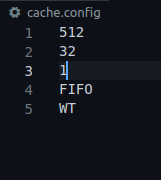
\includegraphics{5_config.png}
    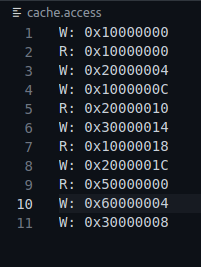
\includegraphics{5_seq.png}
    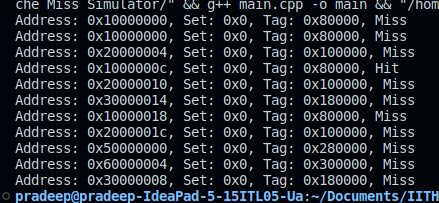
\includegraphics{5_result.png}
    \caption[short]{configuration + Sequence + Result}
\end{figure}

\subsection{Test Case 2: FIFO + Write Through + Fully Associative}
\begin{figure}[H]{\centering}
    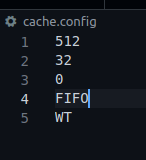
\includegraphics{4_config.png}
    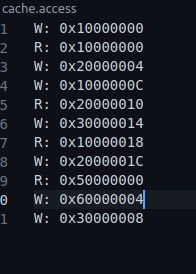
\includegraphics{4_seq.png}
    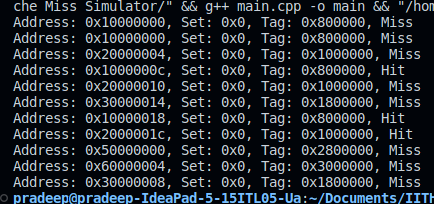
\includegraphics{4_result.png}
    \caption[short]{configuration + Sequence + Result}
\end{figure}

\subsection{Test Case 3: FIFO + Write Through + 4-way Set Associative}
\begin{figure}[H]{\centering}
    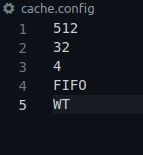
\includegraphics{3_config.png}
    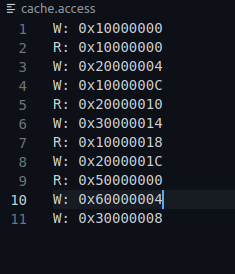
\includegraphics{3_seq.png}
    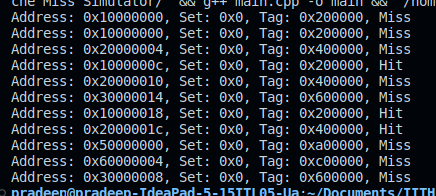
\includegraphics{3_result.png}
    \caption[short]{configuration + Sequence + Result}
\end{figure}

\subsection{Test Case 4: LRU + Write Through + 4-way Set Associative}
\begin{figure}[H]{\centering}
    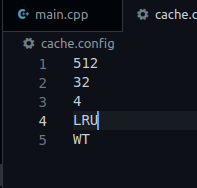
\includegraphics{2_config.png}
    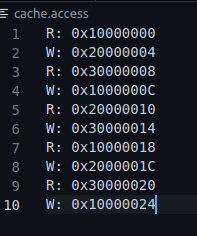
\includegraphics{2_seq.png}
    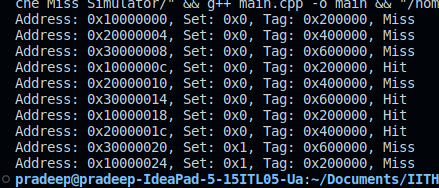
\includegraphics{2_result.png}
    \caption[short]{configuration + Sequence + Result}
\end{figure}

\subsection{Test Case 5: LRU + Write Back + 4-way Set Associative}
\begin{figure}[H]{\centering}
    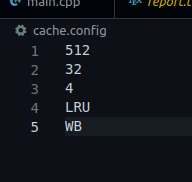
\includegraphics{1_config.png}
    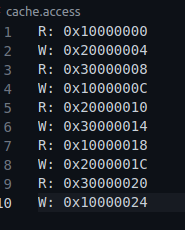
\includegraphics{1_seq.png}
    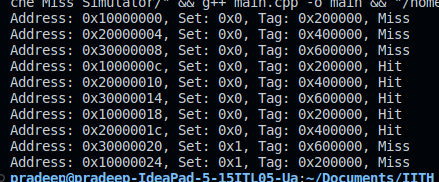
\includegraphics{1_result.png}
    \caption[short]{configuration + Sequence + Result}
\end{figure}

\end{document}
   